\graphicspath{{chapters/4_implementación/figures/}}

\chapter{Implementación}\label{chap:implementation}

La implementación utilizó el lenguaje de programación Rust \cite{rust-lang} y la API de gráficos OpenGL \cite{opengl-spec}.

La arquitectura principal consta de tres paquetes: \textit{cli}, \textit{core} y \textit{engine}.
\textit{Engine} contiene todas las abstracciones sobre OpenGL utilizadas, provee tipos como \textit{Transform}, \textit{Light}, \textit{Camera} que permiten manipular objetos en el espacio 3D.
\textit{Core} contiene todos los algoritmos de voxel cone tracing que hemos mencionado: voxelización, construcción del SVO, filtrado, actualización y el trazado de conos en si.
El paquete \textit{cli} es el punto de entrada de la aplicación, procesa los argumentos pasados por linea de comandos y archivos de configuración y utiliza las funcionalidades expuestas por \textit{engine} y \textit{core} para crear un ambiente 3D con los efectos logrados por voxel cone tracing.
Estos tres paquetes se muestran en la figura \ref{fig:overall_architecture}.

\begin{figure}
    \centering
    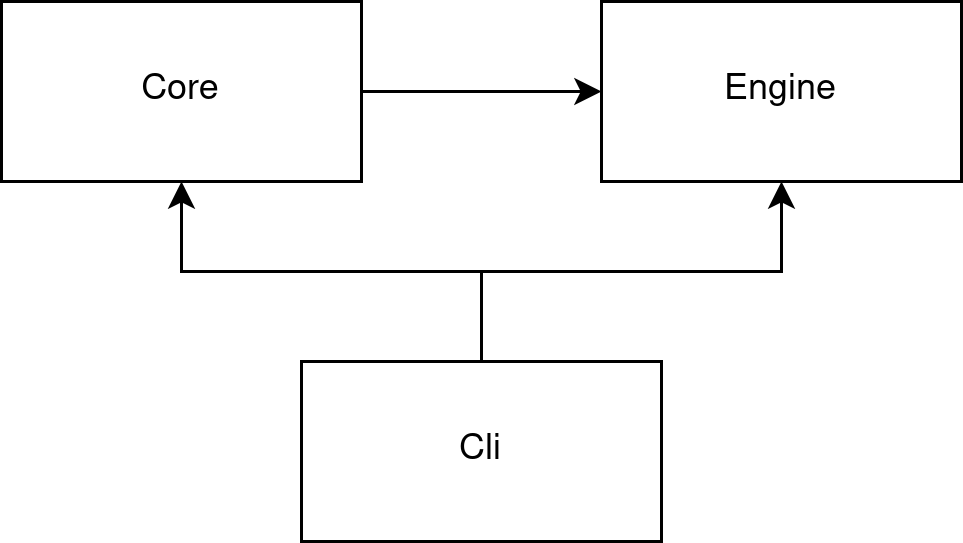
\includegraphics[width=\textwidth]{arquitectura_vct.png}
    \caption{Arquitectura de la implementación}
    \label{fig:overall_architecture}
\end{figure}

En las siguientes secciones se verán a detalle las arquitecturas de cada uno de estos paquetes.

\section{Engine}

Engine expone una serie de abstracciones para interactuar con OpenGL.


\section{Core}

% TODO

\subsection{Representación del SVO}\label{implementation:svo_representation}

La forma de representar este árbol es con una textura lineal en GPU, conocida como la node pool.
Cada texel (píxel de textura) de esta textura es un puntero a otro nodo.
Se toma la convención de que cada grupo de 8 texels es un nodo, cada texel es un puntero al hijo correspondiente.
Los primeros 4 texels representan una subdivisión con valor de $z$ menor mientras que los últimos 4 representan una con valor de $z$ mayor.
Dentro de cada grupo de 4, los primeros 2 son un valor menor de $y$ y los últimos uno mayor.
Dentro de los grupos de 2, primero es menor $x$, último mayor.
Si un texel tiene el valor $0$, entonces ese hijo del nodo no existe.
Si un texel tiene un valor $x != 0$, entonces en la posición $x * 8$ comienza un nuevo nodo, que termina en $x * 8 + 7$.

Cada nodo tiene asociado un brick.
Los bricks son texturas 3D de $3^3$ texels que buscan aproximar la región de la escena que representa el nodo.
Se almacenan en una gran textura 3D llamada la brick pool, con lo cual cada brick es una región de $3^3$ texels de esta gran textura.
Mientras los nodos tienen únicamente punteros a sus hijos, los bricks son los que almacenan los atributos, como el color y la normal.
Cada texel dentro de un brick se llama vóxel, porque además de ser un píxel de textura, también es un píxel de volumen.
Es en estos vóxels que se almacenan los atributos con los que se va a trabajar.

\begin{figure}[h!]
    \centering
    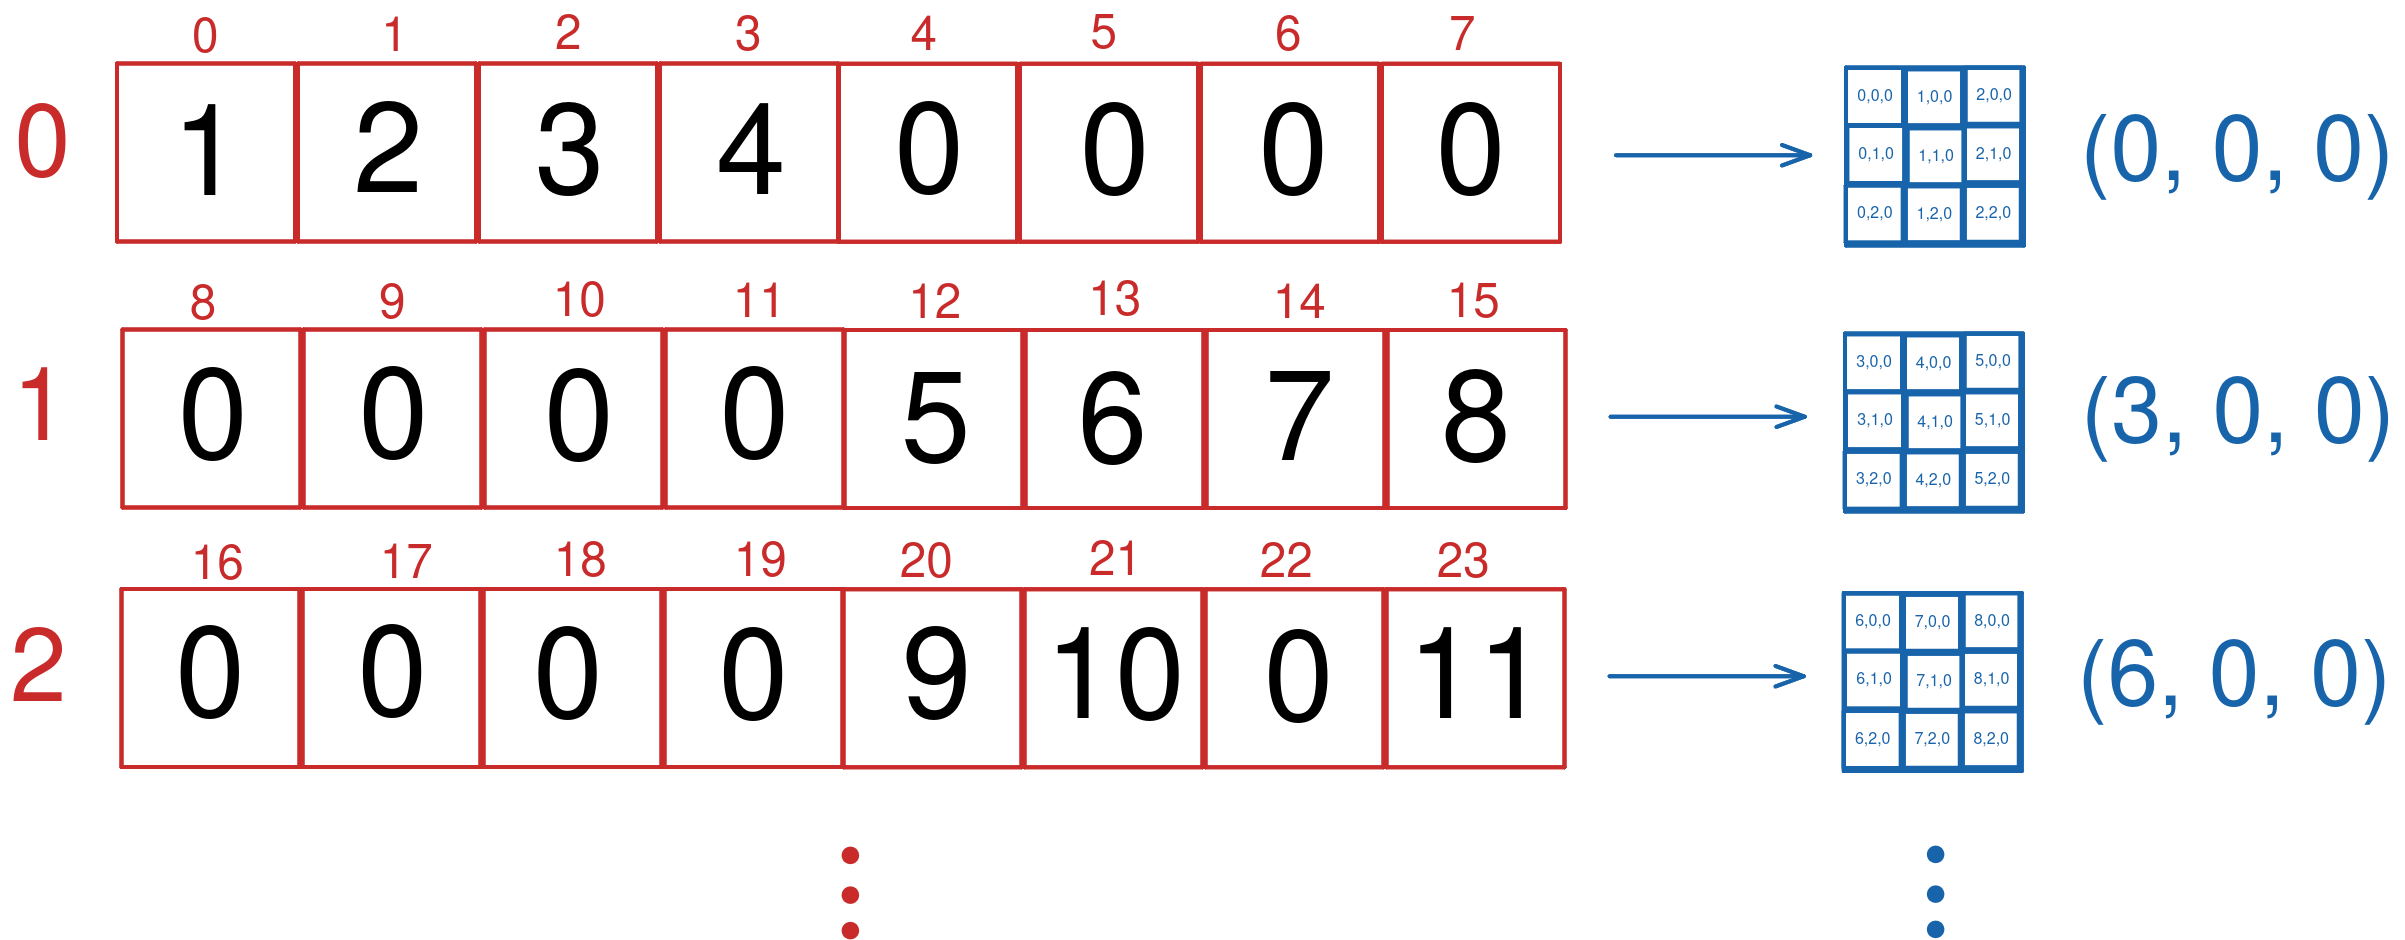
\includegraphics[width=\textwidth]{node-pool-example.png}
    \caption{Ejemplo node pool y brick pool}
    \label{fig:node_pool_example}
\end{figure}

En la figura \ref{fig:node_pool_example} se muestra un ejemplo de node pool y brick pool.
En este ejemplo, vemos que la node pool está pintada de rojo, mientras que la brick pool está pintada de azul.
Cada nodo de la node pool está numerado en el margen izquierdo ($0, 1, 2$), está formado por $8$ texels (los pequeños números arriba de cada caja).
Los números dentro de cada texel de un nodo son los índices del nodo (que debe ser multiplicado por $8$ para conseguir el texel correspondiente) hijo.
Los texels que tienen $0$ indican que esa subdivisión no tiene un hijo.
Acá es donde se ve que la estructura es esparza.

Cada brick es una sección de $3^3$ texels de una gran textura 3D.
Cada nodo tiene asociado un brick, que es identificado únicamente por su índice.
Dado que los bricks existen en una textura 3D, la manera de identificarlos es con un vector de $\mathbb{R}^3$.
Para esto, se usa una función que convierte cada índice de $\mathbb{R}$ en un vector de $\mathbb{R}^3$.

Cada nodo podría tener asociado solo un valor escalar para el atributo que se quiera guardar en él, en lugar de asociarles una textura 3D (el brick).
Sin embargo, usando texturas podemos conseguir los beneficios de la interpolación trilineal provista por el hardware de la GPU al tomar un sample dentro del brick.
Si el sample cae entre dos texels, se interpola.
Esto permite mejorar la calidad de la imagen, como veremos en el capítulo \ref{chap:experiments}.

La node pool y brick pool son la forma en la que se almacenan en memoria los nodos y bricks respectivamente.
Si bien los nodos y los bricks se almacenan usando indices, la región de la escena que representan es totalmente distinta.
Los nodos representan secciones cada vez más chicas de la escena, que resultan de subdividir al nodo padre, ocupando el nodo con indice $0$ toda la escena.
Los bricks se ubican en la escena sobre sus nodos asociados, y se extienden un poco más hacia cada dirección.
Esto es porque los vóxels de los bricks están centrados en los vértices de los nodos.

% TODO: Tuve que mover fig:node_and_brick a diseño porque hay que hablar de nodos y bricks antes.

En la figura \ref{fig:node_and_brick} también se ve la razón por la que los bricks son de tamaño $3^3$, para poder cubrir el espacio del nodo pero también extenderse un poco más allá de su límite.
Esto es necesario para poder conseguir valores de más allá del espacio del nodo y traerlos al brick, así luego, al interpolar los valores dentro del brick, se están teniendo en cuenta valores de una región más grande.
El resultado es que dos nodos vecinos comparten una frontera de vóxels de sus bricks asociados.
Esto se muestra en la figura \ref{fig:brick_border_overlap}.
Dado que estos vóxels representan la misma región del espacio, es necesario que sus valores sean los mismos.
Si bien en memoria son dos entidades distintas que existen en distintos lugares, espacialmente son las mismas, con lo cual debe asegurarse que sus valores sean iguales.

\subsection{Vóxels anisotrópicos}\label{implementation:anisotropic_vóxels}

El cálculo del filtrado anisotrópico requiere conocimiento de los bricks vecinos a la hora de calcular el valor de un vóxel limítrofe.
El shader que realiza el filtrado anisotrópico ejecuta un hilo por brick, con lo cual no se tiene acceso a los bricks vecinos.

Para resolver esto, se carga el vecino en la dirección de filtrado para poder completar los valores direccionales.
Luego se usa un shader que promedia los valores direccionales con los vecinos de las otras dos direcciones.

\subsection{Nodos frontera}\label{implementation:border_nodes}

El procedimiento para producir los nodos frontera reutiliza lo ya existente para generar nodos dado una lista de vóxel fragments\ref{chap:design}, en lugar de modificar directamente con la node pool\ref{chap:design} ya existente.
Al proceso de construcción del octree se le agregan dos pasos:

\begin{itemize}
    \item Construír lista de vóxel fragments
    \item Construir nodos del octree a partir de la lista de vóxel fragments
    \item NUEVO: Construír una lista de vóxel fragments frontera a partir de la lista original de vóxel fragments
    \item NUEVO: Agregar nodos frontera al octree usando la lista de vóxel fragments frontera
\end{itemize}

Se toma la lista de vóxel fragments que fue generada a partir de la geometría de la escena y se hace pasar por un nuevo shader.
Este nuevo shader toma esta lista de vóxel fragments y crea una nueva lista de vóxel fragments ``ficticia'', porque no son parte de la geometría.
Por cada vóxel fragment de la lista original, se recorre el octree y, por cada una de las seis direcciones principales (X, -X, Y, -Y, Z, -Z), se busca si tiene un nodo vecino.
En el caso que no lo tenga, se agrega a la nueva lista un vóxel fragment cuya posición es la del original desplazada hacia la dirección considerada, para que al crearse el nodo en la estructura, este tome el lugar del vecino faltante.

Aprovechar este shader logra que solo sea necesario crear nodos para el último nivel y se subdividen nodos de niveles anteriores automáticamente a medida que se desciende por el árbol.

Una vez se obtiene la nueva lista de vóxel fragments, esta se hace pasar por el mismo shader que convierte vóxel fragments en nodos del octree.
Estos nuevos nodos se agregan al final del buffer de la estructura.
Dado que los nodos nuevos están en distintos niveles, se mantiene una lista de índices distinta para mantener de dónde a dónde va un nivel N en el buffer.

% TODO: Agregar diagramita de como se agregan los nodos frontera al final y se mantienen dos buffers de indices.

\subsection{Menú}

A lo largo de la implementación, fue necesario depurar varios errores y correr pruebas.
Para esto, fue muy útil contar con una interfaz gráfica o menú para seleccionar varias opciones y poder ver valores de la GPU en tiempo real.
Se desarrolló este menú utilizando un paquete del ecosistema de Rust llamado Egui \cite{egui}.

Egui permite rápidamente crear una interfaz gráfica basada en ventanas que se renderiza junto con la aplicación en cada frame.
Es muy sencillo conectar valores del código a etiquetas en el menú y botónes en el menú a acciones.

La herramienta más importante del menú a la hora de depurar fue una ventana que muestra todos los nodos de la node pool.
Esta se puede ver en la figura \ref{fig:node_positions_menu}.
En el menú se muestran todos los nodos de la node pool con su indice (0, 1, 2, ...) y sus coordenadas dentro de la escena (entre 0 y 255).
Al apretar cualquier nodo, se muestra en la escena un cubo delimitando la región de la escena representada por ese nodo.
Se pueden tener muchos nodos mostrándose a la vez.

\begin{figure}
    \centering
    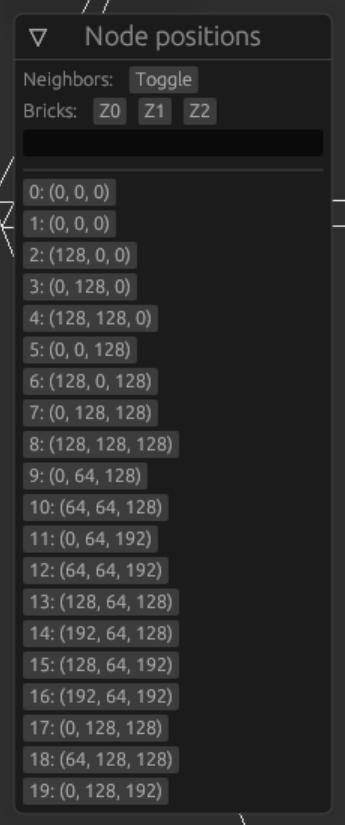
\includegraphics[width=.25\textwidth]{node_positions_menu.png}
    \caption{Menú de nodos}
    \label{fig:node_positions_menu}
\end{figure}

Este menú se puede filtrar, tanto por índice como por coordenadas.
También se pueden mostrar los vecinos de cada nodo y los bricks, que para no llenar la pantalla mucho, se pueden mostrar individualmente cada capa del brick, con $z=0,1,2$.

También se usó la interfaz gráfica para reportar los FPS que fueron usados en el capítulo \ref{chap:experiments} y mostrar otros valores en pantalla, relevantes para el algoritmo.

\section{Cli}

\subsection{Archivos de escena}

Para poder fácilmente cargar distintos modelos y probar el algoritmo en ellos, se creó un formato de archivos de escena.
Estos archivos usan extensión RON, por Rusty Object Notation, una notación similar a JSON, JavaScript Object Notation, pero para Rust.

% TODO: Agregar ejemplos de archivos y qué renderizan

\section{Herramientas} % TODO: Porbablemente buscar de meter esto en otra sección o en la intro del capítulo

\subsection{Rust}

Se eligió el lenguaje de programación Rust para la implementación del algoritmo debido a varias razones:
\begin{itemize}
    \item Es rápido
    \item Tiene un manejador de paquetes por defecto con muchas herramientas disponibles
    \item Tiene una comunidad muy activa y buena documentación
\end{itemize}

Obviamente, se consideró C++ dado que es el lenguaje más popular para aplicaciones gráficas.
El factor que más pesó en la decisión fue la existencia de un manejador de paquetes por defecto.
Esto permitió instalar varias dependencias mucho más rápido y cambiarlas a lo largo del ciclo de desarrollo.

\subsection{OpenGL}

Como se mencionó en el capítulo \ref{chap:design}, el algoritmo fue mayoritariamente implementado en la GPU.
Si bien el lenguaje de programación de la CPU es importante, la elección de la API de gráficos fue, sin duda, la más importante.
Se consideraron Vulkan y CUDA pero se terminó optando por OpenGL debido a varios factores:
\begin{itemize}
    \item Facilidad de desarrollo
    \item Conocimiento previo
    \item Facilidad de trabajo con compute shaders
\end{itemize}

Si bien Vulkan es una API más moderna, el equipo del presente trabajo no contaba con la suficiente experiencia como para utilizarlo adecuadamente, lo cual hubiera llevado a mucho tiempo desperdiciado aprendiendo la herramienta.
CUDA es usualmente utilizado para cálculos arbitrarios en la GPU pero debido a la necesidad de también usar el pipeline gráfico, se optó por usar los compute shaders de OpenGL.
